
\documentclass[9pt, landscape]{article}
\usepackage[utf8]{inputenc}
\usepackage{amsmath}
\usepackage{amsfonts}
\usepackage{amssymb}
\usepackage[ngerman]{babel}
\usepackage{graphicx}
\usepackage{multicol}
\usepackage{geometry}
\usepackage{xcolor}
\usepackage{enumitem}
\usepackage{verbatim}
\usepackage{listings}
\usepackage{booktabs}
\usepackage{tabularx}
\usepackage{ragged2e} % Für besseren Textumbruch in X-Spalten
\usepackage[table]{xcolor}
\usepackage[utf8]{inputenc}
\usepackage[T1]{fontenc}
\usepackage{lmodern}
\usepackage[table]{xcolor}
\usepackage{tabularx}
\usepackage{booktabs}
\usepackage{multirow}
\usepackage{array}
\usepackage{makecell}
\usepackage{titlesec}
\usepackage{etoolbox}
\AtBeginEnvironment{tabularx}{\footnotesize}


% Seitenränder anpassen für maximale Ausnutzung
\geometry{a3paper, left=1.2cm, right=1.2cm, top=1cm, bottom=1cm, landscape}

% --- C++ Style for listings ---
\lstdefinestyle{cpp_style}{
    language=C++,
    basicstyle=\ttfamily\small,
    keywordstyle=\color{blue}\bfseries,
    stringstyle=\color{purple},
    commentstyle=\color{gray},
    numbers=left,
    numberstyle=\tiny\color{gray},
    breaklines=true,
    showstringspaces=false,
    backgroundcolor=\color{lightgray!10} % A very light gray background
}
\lstset{style=cpp_style}

\lstdefinelanguage{ST}{
  morekeywords={VAR,END_VAR,IF,THEN,ELSE,FOR,TO,DO,END_IF,END_FOR, TYPE, STRUCT, END_TYPE, STR, INT, BOOL, REAL, TRUE, FALSE, END_STRUCT, INT, ARRAY, OF, BY, VAR_INPUT, VAR_OUTPUT, VAR_IN_OUT, FUNCTION, FUNCTION_BLOCK, END_FUNCTION, END_FUNCTION_BLOCK, RETURN, CASE, OF, END_CASE, ELSIF},
  sensitive=true,
  morecomment=[l]{(*},
  morecomment=[s]{(*}{*)},
  morestring=[b]",
}
% ST Style ohne Zeilennummern
\lstdefinestyle{st_style}{
    language=ST,
    basicstyle=\ttfamily\small,
    keywordstyle=\color{teal}\bfseries,
    stringstyle=\color{purple},
    commentstyle=\color{gray},
    numbers=none,
    breaklines=true,
    showstringspaces=false,
    backgroundcolor=\color{lightgray!10}
}


\titleformat{\section}
    {\normalfont\large\bfseries} % Kleiner: "large" statt "Large"
    {\thesection}
    {0.7em} % Weniger Abstand nach Nummer
    {}

\titleformat{\subsection}
    {\normalfont\normalsize\bfseries} % Kleiner: "normalsize" statt "large"
    {\thesubsection}
    {0.7em}
    {}

\titlespacing*{\section}
    {0pt}
    {1.0ex plus 0.5ex minus .1ex} % Weniger Abstand davor
    {0.7ex plus .1ex}             % Weniger Abstand danach

\titlespacing*{\subsection}
    {0pt}
    {0.5ex plus 0.2ex minus .1ex}
    {0.5ex plus .1ex}



% Eigene Befehle für Hervorhebungen
\newcommand{\formel}[1]{\ensuremath{#1}}
\newcommand{\algo}[1]{\textbf{\textcolor{blue!60!black}{#1}}}
\newcommand{\datastruct}[1]{\textbf{\textcolor{red!60!black}{#1}}}
\newcommand{\SubItem}[1]{
    {\setlength\itemindent{15pt} \item[-] #1}
}

\setlist{nosep, leftmargin=*}
\setlength{\columnsep}{0.7cm}

\pagestyle{empty}

\begin{document}

\setlength{\columnsep}{5pt}
\begin{multicols*}{4}

\section{Kompilierungsprozess}

\begin{itemize}
    \item \datastruct{Präprozessor}: Führt Direktiven wie \lstinline|#include| und \lstinline|#define| aus. Erzeugt eine erweiterte Quellcodedatei.
    
    \item \datastruct{Compiler}: Übersetzt den C++ Quellcode (\lstinline|.cpp|) in Assembly-Code (\lstinline|.asm|).
   
    \item \datastruct{Assembler}: Folgt auf den Compiler und übersetzt den Assembly-Code in Maschinencode (Binär - \lstinline|.obj|).
   
    \item \datastruct{Linker}: Kombiniert verschiedene Objektdateien und Bibliotheken (\lstinline|.lib|) zu einem einzigen, ausführbaren Programm.

\end{itemize}

\section{Typumwandlung}

\begin{itemize}
    \item \datastruct{Implicit Casting}: Automatische Typumwandlung durch den Compiler.
    \begin{itemize}
        \item \lstinline|int a = 5.4;| $\implies$ a wird zu einem int (5)
        \item \lstinline|float b = 7/2;| $\implies$ Ganzzahlige Division, Ergebnis 3 wird zu double (3.0)
        \item \lstinline|float c = 7/2.0;| $\implies$ Einer der Werte ist float, Ergebnis 3.5
        \item \lstinline|double d = 'A' - 12;| $\implies$ char wird zu int (65), dann - 12 (53), dann zu double (53.0)
        \item \lstinline|int e = true + 3;| $\implies$ bool wird zu int (1) + 3 (4), dann zu int (4)
        \item Allgemein: \textit{Der kleinere Typ wird in den größeren umgewandelt}
    \end{itemize}

    \item \datastruct{Explicit Casting}: Manuelle Typumwandlung durch den Programmierer.
    \begin{itemize} 
        \item \lstinline|int x = (int)3.7;| $\implies$ Klassischer Cast: Ergebnis ist 3
        \item \lstinline|int y = static_cast<int>(3.7);| $\implies$ Moderner Cast mit \lstinline|static_cast|: Ergebnis ist ebenfalls 3
    \end{itemize}
\end{itemize}

\section{Hierarchie von Operatoren}

\noindent % Verhindert Einrückung
\begin{tabularx}{\linewidth}{l l >{\RaggedRight}X}
\toprule
\textbf{Operator} & \textbf{Beschreibung} \\
\midrule
\texttt{x++} & Postfix\\
\texttt{++x} \texttt{*} \textbf{\&} \textbf{!} & Präfix, Ref/Deref, Pointer, NOT (unär) \\
\textbf{* / \%} & Muliplikativ \\
\texttt{+} \texttt{-}  & Additiv  \\
\texttt{<<} \texttt{>>} & Bit-Shift Links(add 0)/Rechts(del 0) \\
\textbf{< > >= <=} & Vergleich \\
\textbf{ == !=} & Gleichheit\\
\texttt{\&}             & Bitweises UND \\
\textbf{\^} & biteweise XOR \\
\texttt{|}             & Bitweises ODER  \\
\texttt{\&\&}            & Binär: Logisches UND \\
\texttt{||}            & Logisches ODER \\
\textbf{= *= += *=} & zusammengesetzte Ausdrücke \\
\bottomrule
\end{tabularx}

\section{Wertebereiche von Datentypen}

\noindent
\begin{tabularx}{\linewidth}{l l >{\RaggedRight}X}
\toprule
\textbf{Datentyp} & \textbf{Bytes} & \textbf{Wertebereich} \\
\midrule
\lstinline|char| & 1 & -128 bis 127 \\
\lstinline|unsigned char| & 1 & 0 bis 255 \\
\lstinline|short| & 2 & -32.768 bis 32.767 \\
\lstinline|unsigned short| & 2 & 0 bis 65.535 \\
\lstinline|int| & 4 & $-2^{31}$ bis $2^{31} -1$ \\
\lstinline|unsigned int| & 4 & 0 bis $2^{32} -1$ \\
\lstinline|long long| & 8 & ca. -9,2 x 10$^{18}$ bis 9,2 x 10$^{18}$ \\
\lstinline|float| & 4 & ca. $\pm$3.4 x 10$^{38}$ (7 Stellen) \\
\lstinline|double| & 8 & ca. $\pm$1.8 x 10$^{308}$ (15 Stelen) \\
\bottomrule
\end{tabularx}

\section{Overflow von Zahlen}
Overflow = Zugewiesene oder berechnete Zahl liegt außerhalb des darstellbaren Bereichs eines Datentyps.
\begin{itemize}
    \item \datastruct{Ganzzahlen}: Undefiniertes Verhalten. z.B. zu hohe Bits werden abgeschnitten oder es wird auf den Minimalwert zurückgesetzt.
    \item \datastruct{Gleitkommazahlen}: Im IEEE 754 Standard wird bei Overflow der Wert \texttt{inf} (unendlich) zugewiesen.
\end{itemize}

\section{Definition und Deklaration}
\begin{itemize}
    \item \algo{Definition}: Reserviert Speicherplatz für eine Variable oder Funktion und kann optional initialisiert werden.
    \begin{itemize}
        \item Beispiel Variable: \lstinline|int x = 5;|
    \end{itemize}
    \item \datastruct{Deklaration}: Informiert den Compiler über den Typ und Namen einer Variable oder Funktion, reserviert aber keinen Speicherplatz.
    \begin{itemize}
        \item Beispiel Variable: \lstinline|extern int x;|
        \item Beispiel Funktion: \lstinline|void foo();|
    \end{itemize}
    \item \datastruct{Prototyp}: Funktionsdeklaration ohne Funktionskörper.
    \begin{itemize}
        \item Beispiel: \lstinline|double sum(double[]);|
    \end{itemize}
    \item \algo{Wichtig}: \textit{Jede Definition ist auch eine Deklaration!}
\end{itemize}

\section{Functional und Lambda}

Benötigt \lstinline|#include <functional>|

\lstinline|std::function<T>| ist nützlich um Funktionen als Objekt zu deklarieren, speichern und übergeben zu können. \algo{Beispiel}:
\lstinline|std::function<int(int,int)> sum = [](int a, int b) { return a + b; };|

\datastruct{Lambda Funktionen}

Lambda Funktionen sind anonyme Funktionen, die direkt im Code definiert werden können. Sie haben die folgende Syntax:

\lstinline|[capture](parameters) -> return_type { body }|

\begin{itemize}
    \item \textbf{Capture}: Bestimmt, welche Variablen aus dem umgebenden Kontext verwendet werden können.
    \begin{itemize}
        \item \lstinline|[]|: Keine Variablen werden erfasst.
        \item \lstinline|[=]|: Alle Variablen werden per Wert erfasst.
        \item \lstinline|[&]|: Alle Variablen werden per Referenz erfasst.
        \item \lstinline|[x, &y]|: Variable \lstinline|x| per Wert \lstinline|y| per Referenz.
    \end{itemize}
\end{itemize}

\section{Iteratoren}
Benötigt \lstinline|#include <vector>|. 
Iteratoren sind Objekte, die verwendet werden, um über die Elemente eines Containers (wie \lstinline|std::vector|, \lstinline|std::list|, etc.) zu iterieren. 
\begin{itemize}
    \item \lstinline|auto it = vec.begin();|: Iterator auf Anfang
    \item \lstinline|auto it = vec.end();|: Iterator hinter das letzte Element
    \item \lstinline|*it|: Zugriff auf Element
    \item \lstinline|++it|, \lstinline|--it|: Vorwärts/Rückwärts bewegen
    \item \lstinline|it != vec.end()|: Vergleich mit Ende
    \item \lstinline|std::advance(it, n)|: Iterator um n Positionen bewegen
    \item \lstinline|std::distance(it1, it2)|: Abstand zwischen zwei Iteratoren
\end{itemize}


 \section{Datenstrukturen Methoden}
\noindent
\begin{tabularx}{\linewidth}{l l >{\RaggedRight}X}
\toprule
\textbf{Typ} & \textbf{Methode} & \textbf{DT} \\
\midrule
v, l, q, s, m & \lstinline|.size()| & size\_t \\
v, l, q, s, m & \lstinline|.empty()| & bool \\
v, l, q & \lstinline|.front()/back()| & T \\
v, l, q& \lstinline|.push_back()/push_front()| & void \\
v, l, q & \lstinline|.pop_back()/pop_front()| & void \\
v, l, m & \lstinline|.begin()/end()| & it \\
l, v & \lstinline|.insert(it,val)| & it  \\
v, l & \lstinline|.clear()| & void \\
s & \lstinline|.top()| & T \\
s & \lstinline|.push()/pop()| & void \\
l & \lstinline|.erase(it)| & it  \\
\bottomrule
\end{tabularx}




 \section{Nützliche std:: Funktionen}
 Benötigt \lstinline|#include <algorithm>| und \lstinline|#include <functional>|

 \noindent
 \begin{tabularx}{\linewidth}{l >{\RaggedRight}X}
 \toprule
 \textbf{Methode} & \textbf{Typ} \\
 \midrule
 \lstinline|std::sort(b, e)| & \lstinline|void| \\
 \lstinline|std::find(b, e, v)| & \lstinline|Iterator| \\
 \lstinline|std::reverse(b, e)| & \lstinline|void|  \\
 \lstinline|std::max(a, b)| & \lstinline|T| \\
 \lstinline|std::find_if(b, e, p)| & \lstinline|Iterator|\\
 \lstinline|std::count_if(b, e, p)| & \lstinline|int|\\
 \lstinline|std::all/any_of(b, e, p)| & \lstinline|bool| \\
 \lstinline|std::max_element(b, e)| & \lstinline|Iterator|\\

 \bottomrule
 \end{tabularx}

 \begin{itemize}
     \item \lstinline|b| = \lstinline|begin()|, \lstinline|e| = \lstinline|end()|
     \item \lstinline|p| = Prädikat (Funktion, die bool zurückgibt) z.B. \lstinline|[](int x){return x>5;}|
     \item \lstinline|v| = Wert, der gesucht wird
     \item \lstinline|d| = Zieliterator (z.B. Anfang eines anderen Containers)
     \item \lstinline|f| = Funktion, die auf jedes Element angewendet wird (z.B. \lstinline|[](int x){return x*2;}|)
 \end{itemize}

\section{Konventionen}

\begin{itemize}
\item \datastruct{Zugriffsmodifikatoren}: Reihenfolge: \lstinline|public:|, \lstinline|protected:|, \lstinline|private:|
\item \datastruct{Konstruktoren}: Immer Explicit angeben 
\item \datastruct{Destruktoren}: Immer Virtual angeben, wenn die Klasse vererbt wird
\item \datastruct{Membervariablen}: Immer mit \lstinline|m\_| oder \lstinline|\_m| kennzeichnen. Keine gleichen Namen wie Parameter im Konstruktor verwenden.
\item \datastruct{Funktionen / Methoden}: Nicht komplett inline definieren: \lstinline|int add(int a, int b) {return a+b}|
\item \datastruct{Void als Parameter}: Nie \lstinline|void| als Parameter verwenden: \lstinline|int foo(void);|
\end{itemize}

\section{Objektorientierung}

\begin{itemize}
   \item \datastruct{Konstruktor / Destruktor}: Konstruktoren werden in verschachtelten Klassen von der innersten zur äußersten Klasse aufgerufen. Destruktoren in umgekehrter Reihenfolge.
   \item \datastruct{Virtual / Overrite}: Virtuelle Funktionen werden in der Basisklasse mit \lstinline|virtual| deklariert und in der abgeleiteten Klasse mit \lstinline|override| überschrieben.
   \begin{itemize}
        \item Wenn eine Methode als \lstinline|virtual| deklariert ist, wird zur Laufzeit die passende Methode der abgeleiteten Klasse aufgerufen, auch wenn der Zeiger oder die Referenz den Typ der Basisklasse hat.
        \item Wenn eine Methode nicht als \lstinline|virtual| deklariert ist, wird die Methode abhängig vom Typ des Zeigers oder der Referenz aufgerufen (statischer Bindung).
   \end{itemize}
   \item \datastruct{Final}: Mit \lstinline|final| kann verhindert werden, dass eine Klasse weiter vererbt wird oder eine Methode überschrieben wird.
\end{itemize}

\section{Smart Pointer}

Smart Pointer sind Klassen, die die Verwaltung von dynamisch allozierten Objekten übernehmen und automatisch den Speicher freigeben, wenn der Pointer nicht mehr benötigt wird.

\begin{itemize}
    \item \lstinline|std::unique_ptr<T>|: Besitzt ein Objekt exklusiv. Kann nicht kopiert, nur verschoben werden. Nutzt \lstinline|std::move()| zum Übertragen des Besitzes.
    \item \lstinline|std::shared_ptr<T>|: Teilt den Besitz eines Objekts mit anderen \lstinline|shared_ptr|s. Verwendet Referenzzählung, um zu wissen, wann das Objekt gelöscht werden kann.
\end{itemize}

\subsection*{make\_shared / make\_unique}

\begingroup\sloppy
Empfohlene Methode zur Erstellung von Smart Pointern; sicherer und effizienter als \lstinline|new|.
\begin{itemize}
    \item \lstinline|auto p = std::make_unique<T>();|
    \item \lstinline|auto p = std::make_shared<T>();| 
    \item optional: Konstruktorparameter in den Klammern
\end{itemize}

\noindent
\begin{tabularx}{\linewidth}{l l}
\toprule
\textbf{Aktion} & \textbf{Code} \\
\midrule
Zugriff auf das Objekt & \lstinline|p->member| \\
Zugriff auf den rohen Zeiger & \lstinline|p.get()| \\
\bottomrule
\end{tabularx}


\endgroup

\subsection*{std::move}
\lstinline|std::move| markiert ein Objekt als "bewegbar", sodass Ressourcen effizient übernommen werden, statt kopiert zu werden. Das Quellobjekt bleibt gültig, aber sein Zustand ist nicht definiert.
\begin{lstlisting}[language=C++]
std::unique_ptr<int> a = std::make_unique<int>(5);
std::unique_ptr<int> b = std::move(a); 
\end{lstlisting}

\noindent
\begin{tabularx}{\linewidth}{l >{\RaggedRight}X}
\toprule
\textbf{Beziehung} & \textbf{Beschreibung } \\
\midrule
\textbf{Assoziation} & ("kennt-ein") Objekte sind unabhängig. \newline
\textbf{C++:} Roher Zeiger (\texttt{*}) oder Referenz (\texttt{\&}), da keine Besitzübernahme. \\

\textbf{Aggregation} & ("hat-ein") Teil-Ganzes, Lebensdauer der Teile ist \textbf{unabhängig}. \newline
\textbf{C++:} \texttt{std::shared\_ptr}, um geteilten Besitz darzustellen. \\


\textbf{Komposition} & ("enthält-ein") Teil-Ganzes, Lebensdauer des Teils ist \textbf{abhängig}. \newline
\textbf{C++:} \texttt{std::unique\_ptr} für exklusiven Besitz oder direktes Member-Objekt. \\
\textbf{Vererbung} & ("ist-ein") Eine Klasse erbt von einer anderen. \\
\bottomrule
\end{tabularx}

\section{Speicherbereiche}

\noindent
\begin{tabularx}{\linewidth}{l >{\RaggedRight}X}
\toprule
\textbf{Bereich} & \textbf{Beschreibung}  \\
\midrule
\textbf{Stack} & Alle Rücksprungadressen und lokalen Variablen  \\
\textbf{Heap} & Dynamisch alloziierte Objekte mit \lstinline|new| oder \lstinline|malloc|  \\
\textbf{Data Segment} & Globale Variablen oder mit \lstinline|static|; zum Programmstart im
Speicher und initialisiert  \\
\textbf{BSS Segment} & Globale Variablen oder mit \lstinline|static|; zum Programmstart im Speicher, aber nicht initialisiert (werden auf 0 gesetzt)  \\

\bottomrule
\end{tabularx}


\textbf{Zugriffszeiten verschiedener Speicherarten}:  Register des Prozessors $>$ Cache Speicher $>$ Hauptspeicher (RAM) $>$ SSD/HDD (Von schnell nach langsam)


\section{Hashing}

\begin{itemize}
    \item \datastruct{Hashmap}: Datenstruktur, die Schlüssel-Wert-Paare speichert und schnellen Zugriff auf Werte über ihre Schlüssel ermöglicht.
    \begin{itemize}
        \item Vorteile: Schneller Zugriff, Einfügen und Löschen in durchschnittlich O(1) Zeit.
    \end{itemize}
    \item \datastruct{Hashfunktion}: Berechnet die Position eines Objektes in einer Tabelle (Array). z.B.:
    \begin{itemize}
        \item \formel{h(k) = k \mod m}, wobei \formel{k} der Schlüssel und \formel{m} die Größe des Arrays ist.
    \end{itemize}
    \item \datastruct{Kollisionsbehandlung}: Methoden zur Behandlung von Kollisionen:
    \begin{itemize}
        \item \algo{Verkettung (Chaining)}: Jedes Array-Element enthält eine Liste von Einträgen, die auf diese Position abgebildet werden.
        \item \algo{Sondieren (Open Addressing)}: Lineares, quadratisches Sondieren oder doppeltes Hashing.
\end{itemize}
\end{itemize}



\subsection*{Beispiele}

\begin{itemize}
    \item \formel{h(k)}: Primäre Hashfunktion (z.B. \formel{k \mod m})
    \item \formel{i}: Anzahl der Versuche (0, 1, 2, ...)
    \item \formel{m}: Größe der Hash-Tabelle
\end{itemize}

\noindent\hrulefill

\begin{itemize} 
\item \datastruct{Lineares Sondieren}: \formel{h_i(k) = (h(k) + i) \mod m}
\item \datastruct{Quadratisches Sondieren}:  \formel{h_i(k) = (h(k) + c_1 \cdot i + c_2 \cdot i^2) \mod m} (meist $c_1 = 0, c_2 = 1$)

\item \datastruct{Doppeltes Hashing}: \formel{h_i(k) = (h(k) + i \cdot h'(k)) \mod m}

\begin{itemize}
    \item \formel{h'(k)}: Zweite Hashfunktion, z.B. \formel{1 + (k \mod m')}, mit \formel{m'} (Primz.) < \formel{m}
\end{itemize}
\end{itemize}

\subsection*{C++ Hashmap}
Benötigt \lstinline|#include <unordered_map>|. \lstinline|std::unordered_map<Key, Value> map;|. \lstinline|std::pair<Key, Value> pair(key, value);|

\noindent
\begin{tabularx}{\linewidth}{l >{\RaggedRight}X}
\toprule
\textbf{Methode} & \textbf{Beschreibung} \\
\midrule
\lstinline|map[key]| & Zugriff/Ändern eines Werts \\
\lstinline|map.insert(\{k,v\})| & Einfügen (pair<it, bool>). Bsp.: \lstinline|auto [it,inserted] = map.insert(...)| \\
\lstinline|map.find(key)| & Sucht Schlüssel, Iterator (\lstinline|it->first|, \lstinline|it->second|) oder \lstinline|end()| \\
\lstinline|map.erase(key)| & Löscht Schlüssel (\lstinline|int| 0 o. 1 Element gelöscht) \\
\bottomrule
\end{tabularx}
\datastruct{Loop}: \lstinline|for(auto [k,v] : map) { ... }|

\section{Vector vs. List}

\noindent
\begin{tabularx}{\linewidth}{l >{\RaggedRight}X}
\toprule
\textbf{Aspekt} & \textbf{Beschreibung} \\
\midrule
\textbf{Speicherstruktur} & \datastruct{Vector}: Kontinuierlicher Speicherblock. \newline \datastruct{List}: Verkettete Knoten, die nicht zusammenhängend im Speicher liegen. \\
\textbf{Zugriffszeit} & \datastruct{Vector}: O(1) für direkten Zugriff. \newline \datastruct{List}: O(n) für direkten Zugriff. \\
\textbf{Einfügen/Löschen} & \datastruct{Vector}: O(n) im Durchschnitt, da Elemente verschoben werden müssen. \newline \datastruct{List}: O(1), wenn der Iterator bekannt ist. \\ 
\textbf{Speicherverbrauch} & \datastruct{Vector}: Weniger Overhead, da nur ein Speicherblock. \newline \datastruct{List}: Mehr Overhead durch Zeiger in jedem Knoten. \\
\bottomrule
\end{tabularx}

\section{Von Neumann Zyklus}
\begin{itemize}
    \item \datastruct{Fetch}: Der Prozessor holt den nächsten Befehl aus dem Speicher (RAM) und lädt ihn in das Befehlsregister.
    \item \datastruct{Decode}: Der Prozessor dekodiert den Befehl, um zu verstehen, welche Operation ausgeführt werden soll und welche Operanden benötigt werden.
    \item \datastruct{Fetch Operands}: Der Prozessor holt die benötigten Operanden aus dem Speicher oder den Registern.
    \item \datastruct{Execute}: Der Prozessor führt die dekodierte Operation aus, indem er die erforderlichen Berechnungen durchführt oder Daten verarbeitet.
    \item \datastruct{Write Back}: Das Ergebnis der Operation wird zurück in den Speicher oder die Register geschrieben.
\end{itemize}

\textbf{Harvard-Architektur}: Getrennte Speicher für Daten und Befehle, paralleler Zugriff möglich.


\section{Automatisierungstechnik}
  \datastruct{Speicherprogrammierbare Steuerung (SPS)}: Industrieller Computer zur Steuerung von Maschinen und Prozessen. SPS-Zyklus:
\begin{itemize}
    \item \algo{Eingabe lesen}: Alle Eingänge (Sensoren, Taster) werden eingelesen (Vom PAE).
    \item \algo{Programm ausführen}: Das Steuerungsprogramm wird basierend auf den Eingaben ausgeführt.
    \item \algo{Ausgabe schreiben}: Alle Ausgänge (Aktoren, Lampen) werden entsprechend dem Programmzustand gesetzt (Vom PAA).
\end{itemize}
\begin{center}
    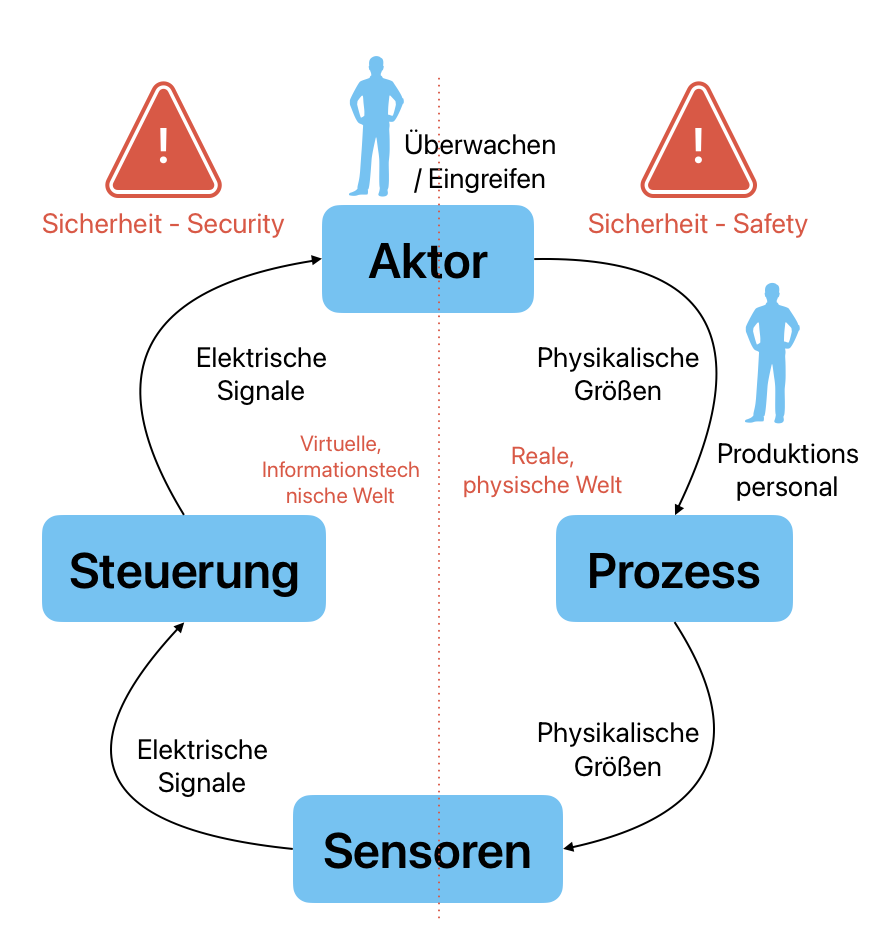
\includegraphics[width=0.8\linewidth]{assets/ATC.png}
\end{center}

\begin{center}
    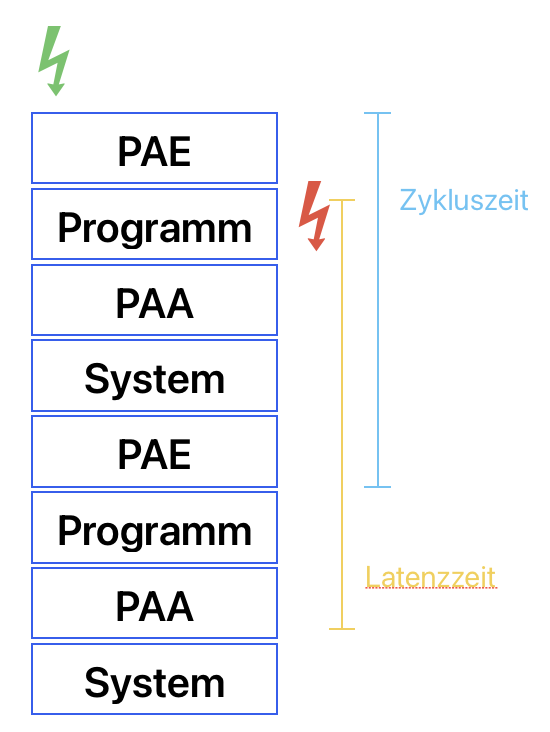
\includegraphics[width=0.5\linewidth]{assets/ATT.png}
\end{center}

\algo{Worst-Case}: Doppelte der Zykluszeit (Eingabe lesen + Programm ausführen + Ausgabe schreiben).

\begin{center}
    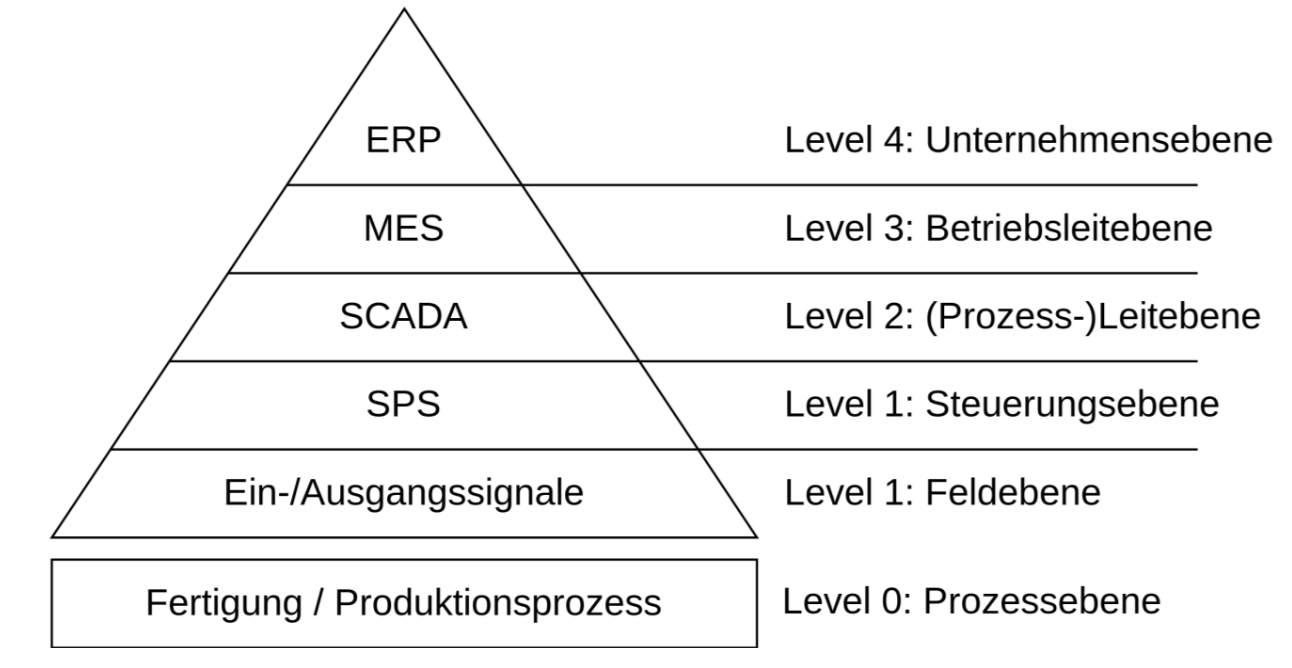
\includegraphics[width=0.8\linewidth]{assets/ATP.png}
\end{center}

\section{Prozessklassifizierung}

\begin{itemize}
    \item \datastruct{Kontinuierliche Prozesse}: Ständige Veränderung der Prozessgrößen (z.B. Temperaturregelung).
    \item \datastruct{Stück-Prozesse}: Verarbeitung einzelner Einheiten (z.B. Montage von Autos).
    \item \datastruct{Batch-Prozesse}: Verarbeitung in Chargen (z.B. Chemische Produktion).
\end{itemize}

\section{IEC 61131-3}
Deklaration von Variablen:

\begin{lstlisting}[language=ST, numbers=none]
TYPE Ampel :
STRUCT
    AKTIV         : BOOL;
END_STRUCT
END_TYPE
TYPE AmpelArray : ARRAY[1..3] OF Ampel; END_TYPE
VAR
    Hauptstr_Ampel : Ampel;
    Zykluszeit     : TIME := T#5s;
    AlleAmpeln     : AmpelArray;
END_VAR
\end{lstlisting}

\algo{Hinweis}: \textit{Variablen können auch in \lstinline|VAR_GLOBAL ... END_VAR| Blöcken deklariert werden, um sie in mehreren Programmen verfügbar zu machen.}

\begin{itemize}
\item \algo{Kontaktplan}: Grafische Programmiersprache, die elektrische Schaltpläne nachbildet.
\begin{itemize}
    \item \texttt{--][--}: Schließer
    \item \texttt{--]\textbackslash{}[--}: Öffner
    \item \texttt{--()\!--}: Spule (Aktor)
\end{itemize}
\item \algo{Funktionsbausteinsprache (FBS)}: Logik-Gatter, FlipFlops, TON, TOF werden als Bausteine dargestellt und verbunden.
\item \algo{Continuous Function Chart (CFC)}: Erweiterung der FBS mit freier Anordnung der Bausteine. Keine strikte Abarbeitung von links nach rechts.
\item \algo{Strukturierter Text (ST)}: Hochsprachliche Programmiersprache ähnlich zu Pascal/C. Syntax: 

\begingroup\sloppy
\begin{itemize}
    \item Variablen mit \lstinline|VAR ... END_VAR| deklarieren
    \item Anweisungen mit \lstinline|:=| für Zuweisung
    \item Kontrollstrukturen: \lstinline|IF ... THEN ... ELSE ... END_IF;|, \lstinline|FOR ... TO ... DO ... END_FOR;|
    \item Funktionen und Funktionsbausteine mit \lstinline|FUNCTION ... END_FUNCTION| bzw. \lstinline|FUNCTION_BLOCK ... END_FUNCTION_BLOCK|
\end{itemize}
\endgroup

\begin{lstlisting}[language=ST, numbers=none]
FOR i := 1 TO 3 BY 1 DO
    AlleAmpeln[i].AKTIV := FALSE;;
END_FOR;

IF Hauptstr_Ampel.AKTIV THEN
    Nebenstr_Ampel.L_ROT := TRUE;
ELSIF NOT Hauptstr_Ampel.AKTIV THEN
    Nebenstr_Ampel.L_GRUEN := TRUE;
END_IF;
\end{lstlisting}
\item \algo{Ablaufsprache (AS)}: Grafische Sprache für Zustände und Übergänge; ideal für Ablaufsteuerungen.
\textbf{Aktionen}: 
\noindent
\begin{tabularx}{\linewidth}{l >{\RaggedRight}X}
\toprule
\textbf{BZ} & \textbf{Beschreibung}  \\
\midrule
\textbf{N} & 1 im aktuellen Zustand  \\
\textbf{R} & Reset (auf 0 setzen)  \\
\textbf{S} & Set (auf 1 setzen)  \\
\textbf{P} & 1 nach einem Übergang von 0 zu 1  \\
\textbf{L} & 1 bis Zeit abgelaufen  \\
\textbf{D} & 1 nach Zeitverzögerung  \\
\bottomrule
\end{tabularx}
\end{itemize}

\subsection*{Alternativ vs. Parallel}

\begin{itemize}
    \item \algo{Alternativ}: Nur ein Pfad wird ausgeführt. Übergänge mit Bedingungen.
    \item \algo{Parallel}: Mehrere Pfade werden gleichzeitig ausgeführt. Synchronisation durch spezielle Übergänge.
\end{itemize}

\section{Objektorientierung (AT)}
\begin{itemize}
    \item \datastruct{Datenkapselung}: mit GET und SET Methoden.
    \item \datastruct{Vererbung}: Mit \lstinline|EXTENDS| Schlüsselwort.
    \item \datastruct{Interfaces}: Mit \lstinline|INTERFACE ... END_INTERFACE| Blöcken.
\item \datastruct{Funktionsblöcke}: {\sloppy Mit \lstinline|FUNCTION_BLOCK ... END_FUNCTION_BLOCK| Blöcken.}
    \begin{lstlisting}[language=ST, numbers=none]
FUNCTION_BLOCK Fun
VAR_INPUT in : INT; END_VAR
VAR_OUTPUT out : INT; END_VAR
out = in * 2;
END_FUNCTION_BLOCK

Fun(in := 5, out => result);

    \end{lstlisting}
\end{itemize}

\section{Automatisierungsarchitekturen}

\begin{itemize}
    \item \datastruct{Zentral}: Eine SPS steuert alles.
    \item \datastruct{Dezentral}: Mehrere SPS teilen Aufgaben (Hohe verlässigkeit $\implies$ Kein Gesamtausfall).
    \item \datastruct{Verteilt}: Steuerung über Netzwerk verteilt.
    \item \datastruct{Hierarchisch}: Steuerung auf mehreren Ebenen.
\end{itemize}

\section{Redundanz und Fehler}

\begin{itemize}
\item \algo{Redundanz}: Mehrfache Ausführung von kritischen Komponenten.
\begin{itemize}
    \item \datastruct{Hardware-Redundanz}: Mehrere SPS, Sensoren, Aktoren.
    \item \datastruct{Software-Redundanz}: Mehrere Programme oder Algorithmen für dieselbe Aufgabe.
    \item \datastruct{Zeit-Redundanz}: mehrfache Abfrage des gleichen Messwertes in bestimmten Zeitabständen.
\end{itemize}
%\item \algo{Verfügbarkeit}: Beschreibt, wie häufig oder zuverlässig es betriebsbereit ist.
%\item \algo{Sicherheit}: Fähigkeit eines Systems, gefährliche Fehler zu erkennen und in einen sicheren Zustand zu überführen. 

\end{itemize}

\section{Sicherheits-Integritätslevel}
Das SIL gibt die erforderliche Risikominderung für sicherheitsbezogene Systeme an.

\noindent
\begin{tabularx}{\linewidth}{l >{\RaggedRight}X}
\toprule
\textbf{SIL} & \textbf{Beschreibung}  \\
\midrule
\textbf{SIL 1} & Niedrigste Stufe. Relativ hohe Fehlerwahrscheinlichkeit akzeptiert. Für geringe Risiken, z.B. einfache Alarmsysteme. \\
\textbf{SIL 2} & Mittlere Stufe. Erhöhte Zuverlässigkeit nötig. Für Anwendungen mit moderatem Gefahrenpotenzial, z.B. Not-Aus-Schalter. \\
\textbf{SIL 3} & Hohe Stufe. Sehr geringe Fehlerwahrscheinlichkeit. Für schwere Verletzungsgefahr, z.B. Sicherheitsbarrieren, Zugsteuerungen. \\
\textbf{SIL 4} & Höchste Stufe. Extrem geringe Fehlerwahrscheinlichkeit. Für extrem kritische Systeme, z.B. Kernkraftwerke, Flugzeugsteuerungen. \\
\bottomrule
\end{tabularx}

Das SIL ergibt sich aus einer Risikoanalyse: Schwere (S), Häufigkeit (F), Wahrscheinlichkeit (W), Vermeidbarkeit (P).
\algo{Safty Inegrated Function}: Besteht aus: Sensorik (Fehler erkennen), Logik (SPS - Fehler bewerten) und Aktorik (Sicheren Zustand einleiten).

\section{MooN Architektur}
Es müssen mindestens $M$ von insgesamt $N$ Komponenten korrekt funktionieren, damit das System eine
sicherheitsrelevante Aktion ausführt. 

\noindent
\begingroup
\setlength{\tabcolsep}{4pt}
\renewcommand{\cellalign}{l} % Stellt sicher, dass der Text in makecell linksbündig ist
\begin{tabularx}{\linewidth}{l >{\RaggedRight}X  >{\RaggedRight}X}
\toprule
\textbf{Architektur} &  \textbf{Sicherheit / Verfügbarkeit} & \textbf{Anwendung} \\
\midrule
\textbf{1oo1} &  Niedrig / Hoch & Einfache Steuerungen \\
\textbf{1oo2} & Mittel / Hoch & Prozessüberwachung mit Alarm \\ % Hier wird der Befehl verwendet
\textbf{1oo2D} & Hoch / Hoch & SIL 2-3 Anwendungen \\
\textbf{2oo2} & Sehr Hoch / Niedrig & Not-Aus, Reaktorschutz \\
\textbf{2oo3} & Hoch / Hoch & Kritische Systeme \\
\textbf{3oo3} & Extrem Hoch / Sehr niedrig & SIL-4 Anwendungen \\
\bottomrule
\end{tabularx}
\endgroup

\end{multicols*}
\end{document}

